\chapter{Introduction to Wireless Sensor Networks}



This chapter gives a brief introduction into Wireless Sensor Networks (WSNs)
and its components - wireless sensor nodes. Additionaly, it presents WSN protocol stack 
and gives a short overview over WSN routing techniques.


\section{Sensor Nodes} \label{subsec:sensornodes}
WSNs are typically deployed randomly in a possibly
large area where phenomena are required to be monitored, and consist of the
large number of the light-weighted and tiny devices that can be
easily deployed, called \emph{Sensor Nodes}. 

Typically, a sensor node consists of the following elements (as it can be seen
from the Figure \ref{Fig:SensorNodeArch})
\begin{itemize}
  \item \emph{Sensing unit}, which is comprised of a number of sensors and
  analog-to-digital converters. 
  \item \emph{Tranceiver}, which facilitates node-node communication using 
a variety of techniques.
  \item \emph{Processing unit}, that usually comprises a 
microcontroller/microprocessor that performs processing, and is associated with 
a storage unit.
  \item \emph{Power unit}, which provides the energy required to run the sensor node, and can use chemical 
batteries or power scavenging units such as solar cells.
\end{itemize}

\begin{figure}[h]
\centering
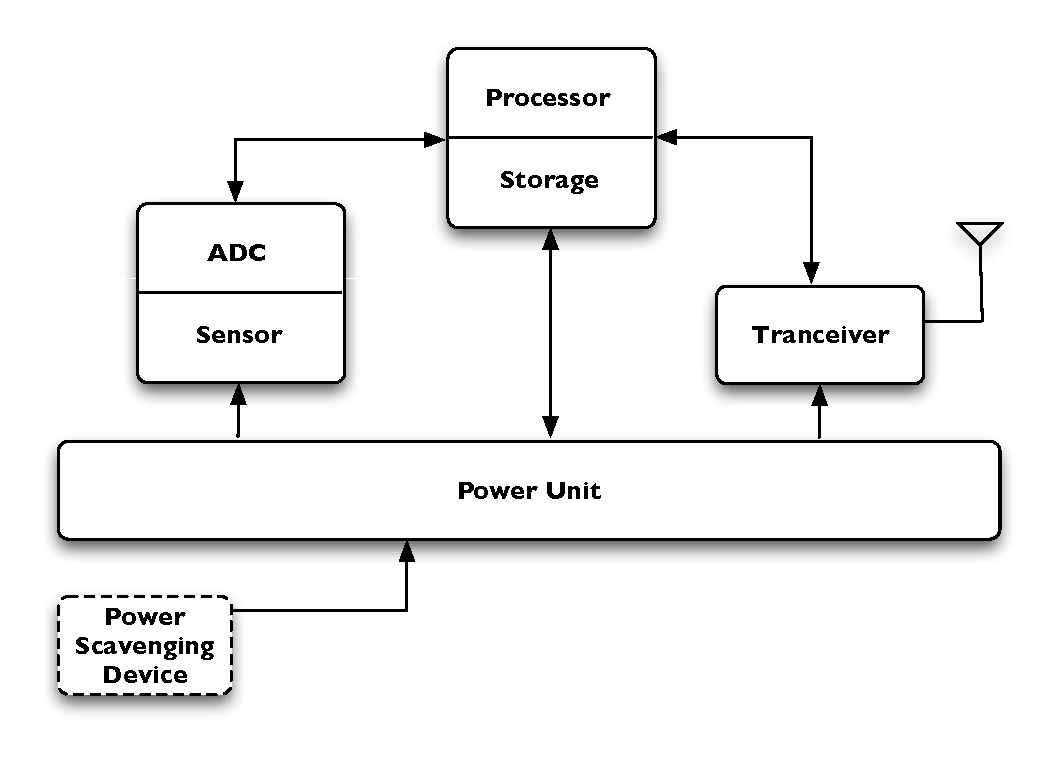
\includegraphics[scale=0.65]{img/SensorNodeArch.eps} 
\caption[Architecture of a sensor node] {Architecture of a sensor node (adapted from \cite{SensorSurveyAkyildiz:2002}).}
\label{Fig:SensorNodeArch}
\end{figure} 

Due to the small size of the devices, sensor nodes have a number of constraints
which affect the WSN built on top of it, among those are \cite{yao:qps}:
\begin{itemize}
  \item \emph{Power consumption constraint} due to the fact that sensor nodes
  have limited energy supply, therefore energy conservation is the main concern when
  WSN applications are implemented.
  \item \emph{Computation restriction} which is caused by the limited memory
  capacity and processing power available on the sensor node, thus possibilities to
  use data processing algorithms on a node are seriously limited. 
  \item \emph{Communication constraint} is caused by the minimal bandwidth and a
  limited quality of service provided by the sensor node's hardware. 
\end{itemize}

Additionally, the deployment of sensor nodes in the WSNs should be
cost-effective, and therefore cost of a single device is a supplementary constraint.

A WSN is self-organising system, given the random nature of the deployment. Its
topology is subject to change, and therefore sensor nodes should be capable of
dealing with changes of this kind in order to cope with hostile operating
conditions, the failure-prone nature of sensor nodes and the possibility of
redeployment of additional sensor nodes at any time during operation.

\section{WSN Protocol Stack} \label{sec:WSNProtStack}

\begin{figure}[h]
\centering
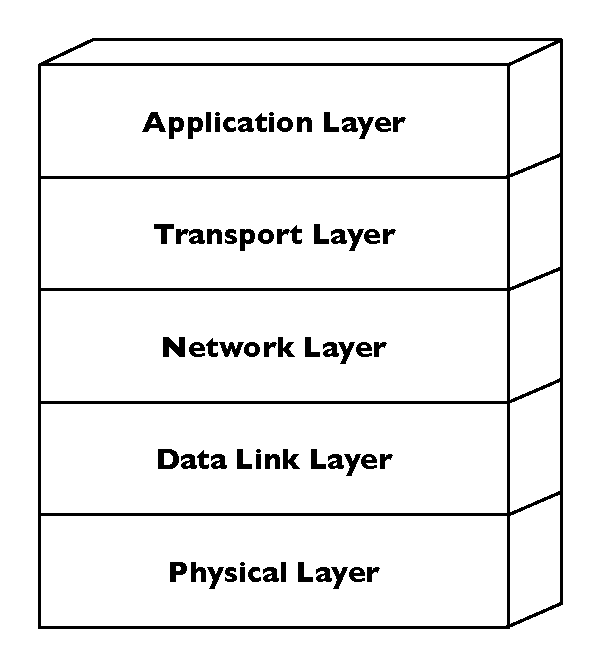
\includegraphics[scale=0.65]{img/ProtStack.eps}
\caption[WSN protocol stack]{WSN protocol stack (reproduced from \cite{SensorSurveyAkyildiz:2002})}
\label{Fig:ProtStack}
\end{figure}

The WSN protocol stack that was presented in \cite{SensorSurveyAkyildiz:2002}
is an adapted generic protocol stack \cite{ComputerNetworksTannenbaum:2003}. As
it can be seen from the Figure \ref{Fig:ProtStack}, the WSN protocol stack consists of the following layers:

\begin{itemize}
\item \emph{Physical Layer}, which provides the transmission of data over the physical transmission medium.
\item \emph{Data Link Layer}, which deals with power-aware Medium Access Control (MAC) protocols that minimise collisions and transceiver on-time.
\item \emph{Network Layer}, which is primarily responsible for
routing data across the network.
\item \emph{Transport Layer}, which provides reliable delivering of data and
supports error checking mechanisms.
\item \emph{Application Layer}, where the application software is resided.
\end{itemize}

\section {Routing in WSNs}
\textcolor{red}{add brief overview of routing techniques}